\usepackage{etex} %эта магическая херь избавляет от переполнения регистров TeX а!!!

\mode<article>{\usepackage{fullpage}}
\mode<presentation>{
    \usetheme{Madrid}
    \useoutertheme{shadow}
} 

\usepackage[utf8]{inputenc}
\usepackage[russian]{babel}
\usepackage{indentfirst}
\usepackage{graphicx}

\usepackage{amsmath}
\usepackage{amsfonts}
\usepackage{amsthm}
%\usepackage{algorithm}
%\usepackage{algorithmic}

%\usepackage[all]{xy}

\date{Лекция по дисциплине <<методы и средства защиты компьютерной информации>> (\today)}
\author[М.~М.~Шихов]{Михаил Шихов \\ \texttt{\underline{m.m.shihov@gmail.com}}}

%%для рисования графов пакетом xy-pic
%\entrymodifiers={++[o][F-]}

%%для псевдокода алгоритмов (algorithm,algorithmic)
%\renewcommand{\algorithmicrequire}{\textbf{Вход:}}
%\renewcommand{\algorithmicensure}{\textbf{Выход:}}
%\renewcommand{\algorithmiccomment}[1]{// #1}
%\floatname{algorithm}{Псевдокод}

%\setbeamercolor{alerted text}{fg=-green} %gyan, blue, green, -green


\title[Орг-тех методы]{Организационно-технические методы защиты информации.}


\begin{document}


%титул и содержание статьи
\mode<article>{\maketitle\tableofcontents}

%титул и содержание презентации
\frame<presentation>{\titlepage}
\begin{frame}<presentation>
\frametitle{Содержание}
\tableofcontents
\end{frame}


\section{Информационная безопасность}


\begin{frame}
\frametitle{Информационная безопасность}
\begin{definition}%theorem, lemma, proof, corollary, example
Под \alert{информационной безопасностью (ИБ)} понимают защищенность инофрмации от незаконного ознакомления, преобразования и уничтожения, а также защищенность информационных ресурсов от воздействий, направленных на нарушение их работоспособности.
\end{definition}
\end{frame}

Основным элементом создания, получения, накопления, передачи, обработки и уничтожения является автоматизированная система обработки информации (АС).

\begin{frame}
\frametitle{Компоненты АС}
Компоненты автоматизированной системы обработки информации можно разбить на следующие группы:
\begin{itemize}
    \item аппаратные средства;
    \item программные средства;
    \item данные;
    \item персонал;
    \item пользователи;
\end{itemize}
\end{frame}

Важной частью АС является система безопасности.

\begin{frame}
\frametitle{Три компонента подсистемы безопасности АС}
\begin{itemize}
    \item Оборона --- противодействие атаке.
    \item Сдерживание --- регламент, противодействие переходу от угрозе к атаке.
    \item Обнаружение --- выявление угроз, а также происходящих или прошедших незамеченными атак с целью анализа порождаемых угроз или угроз эти атаки повлекших.
\end{itemize}
\end{frame}

С точки зрения системы безопасности компоненты АС можно разделить на две больших группы.

\begin{frame}
\frametitle{Разделение сущностей АС}
\begin{itemize}
    \item Субъекты --- активные компоненты, воздействующие на объекты или другие субъекты. Пользователи, персонал, процессы, задачи, потоки. Субъект, подвергаясь воздействию становится объектом.
    \item Объекты --- пассивные компоненты, подвергающиеся воздействию со стороны субъектов. Носители, контейнеры, файлы, каналы передачи.
\end{itemize}
\end{frame}

В рамках АС все объекты должны быть идентифицированы, а субъекты дополнительно еще и аутентифицированы.
Нормативные и методические документы РФ выдвигают требования обеспечению ИБ.

\subsection[Требования к обеспечению ИБ]{Требования к обеспечению информационной безопасности}

\begin{frame}
\frametitle{Основные требования к обеспечению информационной безопасности}
\begin{itemize}
\item Информационная безопасность основывается на положениях и  требованиях существующих законов, стандартов и нормативно-методических документов.
\item Информационная безопасность обеспечивается комплексом программно-технических средств и поддерживающих их организационных мер.
\item Информационная безопасность должна обеспечиваться на всех технологических этапах обработки информации и во всех режимах функционирования, в том числе при проведении ремонтных и регламентных работ.
\end{itemize}
\end{frame}


\begin{frame}
\frametitle{Основные требования к обеспечению информационной безопасности}
\begin{itemize}
\item Программно-технические средства защиты не должны существенно ухудшать основные функциональные характеристики информационной системы (надежность, быстродействие, возможность изменения конфигурации).
\item Оценка эффективности средств защиты информационной системы, учитывающая всю совокупность её технических и проектных характеристик, а также практическую реализацию средств защиты, должна быть неотъемлемой частью работ по обеспечению информационной безопасности.
\item Защита должна предусматривать контроль эффективности средств защиты. Этот контроль может быть периодическим либо инициироваться в рамках мер по обнаружению угроз и атак.
\end{itemize}
\end{frame}


Исходя из методических документов, требования к обеспечению информационной безопасности могут быть реализованы при условии соблюдения ряда принципов.


\subsection[Принципы обеспечения ИБ]{Принципы обеспечения информационной безопасности}

\begin{frame}
\frametitle{Основные принципы обеспечения информационной безопасности}
\begin{itemize}
\item Системности.
\item Комплексности.
\item Непрерывности защиты.
\item Разумной достаточности.
\item Гибкости управления и применения.
\item Открытости алгоритмов и механизмов защиты.
\item Простоты применения защитных мер и средств.
\end{itemize}
\end{frame}

Раскроем суть изложенных принципов.

\begin{itemize}
\item Принцип системности

Системный подход к защите компьютерных систем предполагает необходимость учета всех взаимосвязанных, взаимодействующих и изменяющихся во времени элементов, условий и факторов:
\begin{itemize}
\item при всех видах информационной деятельности и информационного проявления;
\item во всех структурных элементах;
\item при всех режимах функционирования;
\item на всех этапах жизненного цикла;
\item с учетом взаимодействия объекта защиты с внешней средой.
\end{itemize}

При обеспечении информационной безопасности АС необходимо учитывать все слабые, наиболее уязвимые места системы обработки информации, а также характер, возможные объекты и направления атак на систему со стороны нарушителей (особенно высококвалифицированных злоумышленников), пути проникновения в распределенные системы и несанкционированного доступа (НСД) к информации. Система защиты должна строиться не только с учетом всех известных каналов проникновения, но и с учетом возможности появления принципиально новых путей реализации угроз безопасности.

\item Принцип комплексности

Современные средства вычислительной техники, операционные системы, инструментальные и прикладные программные средства обладают множеством встроенных элементов защиты. Комплексное их использование предполагает согласование разнородных средств при построении целостной системы защиты, перекрывающей значительную часть множества возможностей реализации угроз и не содержащей слабых мест на стыках отдельных ее компонентов.

\item Принцип непрерывности защиты

Защита информации - это не разовое мероприятие и даже не конкретная совокупность уже проведенных мероприятий и установленных средств защиты, а непрерывный целенаправленный процесс, предполагающий принятие соответствующих мер на всех этапах жизненного цикла АС (начиная с самых ранних стадий проектирования, а не только на этапе ее эксплуатации). Разработка системы защиты должна вестись параллельно с разработкой самой защищаемой системы. Это позволит учесть требования безопасности при проектировании архитектуры и, в конечном счете, позволит создать более эффективные (как по затратам ресурсов, так и по стойкости) защищенные системы. Большинству физических и технических средств защиты для эффективного выполнения своих функций необходима постоянная организационная (административная) поддержка (своевременная смена и обеспечение правильного хранения и применения имен, паролей, ключей шифрования, переопределение полномочий и т.д.). Перерывы в работе средств защиты могут быть использованы злоумышленниками для анализа применяемых методов и средств защиты, внедрения специальных программных и аппаратных "закладок" и других средств преодоления системы защиты после восстановления ее функционирования.

\item Разумная достаточность

Создать абсолютно непреодолимую систему защиты принципиально невозможно: при достаточных времени и средствах можно преодолеть любую защиту. Например, средства криптографической защиты в большинстве случаев не гарантируют абсолютную стойкость, а обеспечивают конфиденциальность информации при использовании для дешифрования современных вычислительных средств в течение приемлемого для защищающейся стороны времени. Поэтому имеет смысл вести речь только о некотором приемлемом уровне безопасности (Как нужно бежать от медведя? \footnote{Если вы с другом бежите от медведя, то вам нужно бежать не быстрее медведя, а быстрее друга}). Высокоэффективная система защиты стоит дорого, использует при работе существенную часть мощности и ресурсов компьютерной системы и может создавать ощутимые дополнительные неудобства пользователям. Важно правильно выбрать тот достаточный уровень зашиты, при котором затраты, риск и размер возможного ущерба были бы приемлемыми (задача анализа риска). Гибкость системы защиты. Часто приходится создавать систему защиты в условиях большой неопределенности. Поэтому принятые меры и установленные средства защиты, особенно в начальный период их эксплуатации, могут обеспечивать как чрезмерный, так и недостаточный уровень защиты. Естественно, что для обеспечения возможности варьирования уровнем защищенности средства защиты должны обладать определенной гибкостью. Особенно важно это свойство в тех случаях, когда средства защиты необходимо устанавливать на работающую систему, не нарушая процесс ее нормального функционирования. Кроме того, внешние условия и требования с течением времени меняются. В таких ситуациях свойство гибкости спасает владельцев АС от необходимости принятия кардинальных мер по полной замене средств защиты на новые.

\item Открытость алгоритмов и механизмов защиты
Суть принципа открытости алгоритмов и механизмов защиты состоит в том, что защита не должна обеспечиваться только за счет секретности структурной организации и алгоритмов функционирования ее подсистем - Знание алгоритмов работы системы защиты не должно давать возможности ее преодоления (даже автору). Однако это вовсе не означает, что информация о конкретной системе защиты должна быть общедоступна. Необходимо обеспечивать защиту от угрозы раскрытия параметров системы.

\item Принцип простоты применения средств защиты

Механизмы защиты должны быть интуитивно понятны и просты в использовании. Применение средств защиты не должно быть связано со знанием специальных языков или с выполнением действий, требующих значительных дополнительных трудозатрат при обычной работе законных пользователей, а также не должно требовать от пользователя выполнения рутинных малопонятных ему операций (ввод нескольких паролей и имен и т.д.).

\end{itemize}


\section{Политика информационной безопасности}

При принятии решений администраторы информационных систем сталкиваются с проблемой выбора вариантов решений по организации защиты информации на основе учета принципов деятельности организации, соотношения важности целей и наличия ресурсов. Эти решения включают определение того, как будут защищаться технические и информационные ресурсы, а также как должны вести себя служащие в тех или иных ситуациях.

\begin{frame}
\frametitle{Политика информационной безопасности}
\begin{definition}%theorem, lemma, proof, corollary, example
\alert{Политика информационной безопасности (ПИБ)} --- это набор законов, правил, практических рекомендаций и практического опыта, определяющих управленческие и проектные решения в области защиты информации.
\end{definition}
\end{frame}

На основе ПИБ строится управление, защита и распределение критичной информации в системе. Она должна охватывать все особенности процесса обработки информации, определяя поведение информационной системы в различных ситуациях. Для конкретной АС политика безопасности должна быть индивидуальной. Она зависит от технологии обработки информации, используемых программных и технических средств, структуры организации и т.д.

\begin{frame}
\frametitle{Основные направления защиты, охватываемые политикой}
\begin{itemize}
    \item защита объектов информационной системы;
    \item защита процессов, процедур и программ обработки информации;
    \item защита каналов связи;
    \item подавление побочных электромагнитных излучений;
    \item управление системой защиты.
\end{itemize}
\end{frame}

Очевидно, что каждое из указанных направлений должно быть детализировано в зависимости от особенностей структуры ИС.

Кроме этого ПИБ должна описывать и этапы создания системы защиты.

\begin{frame}
\frametitle{Этапы создания системы защиты}
\begin{itemize}
    \item определение информационных и технических ресурсов, подлежащих защите;
    \item выявление полного множества потенциально возможных угроз и каналов утечки информации;
    \item проведение оценки уязвимости и рисков информации на выявленном множестве угроз и каналов утечки;
    \item определение требований к системе защиты;
    \item осуществление выбора средств защиты информации и их характеристик;
    \item внедрение и организация использования выбранных мер, способов и средств защиты;
    \item осуществление контроля целостности и управление системой защиты.
\end{itemize}
\end{frame}

Политика безопасности определяется как совокупность документированных управленческих решений, направленных на защиту информации и ассоциированных с ней ресурсов. При разработке и проведении ее в жизнь целесообразно руководствоваться определенными принципами.

\begin{frame}
\frametitle{Принципы политики безопасности}
\begin{itemize}
    \item невозможность миновать защитные средства;
    \item усиление самого слабого звена;
    \item недопустимость перехода системы защиты в небезопасное состояние;
    \item минимизация привилегий;
    \item разделение обязанностей;
    \item многоуровневая защита;
    \item разнообразие защитных средств;
    \item простота и управляемость информационной системы;
    \item обеспечение всеобщей поддержки мер безопасности.
\end{itemize}
\end{frame}

Раскроем смысл изложенных принципов.

\begin{itemize}

\item Принцип невозможности миновать защитные средства означает, что все информационные потоки в защищаемую сеть и из нее должны проходить через СЗИ. Например, не должно быть <<тайных>> модемных входов или тестовых линий, идущих в обход экрана.

\item Надежность любой СЗИ определяется самым \alert{слабым звеном}. Часто таким звеном оказывается не компьютер или программа, а человек, и тогда проблема обеспечения информационной безопасности приобретает нетехнический характер.

\item Принцип недопустимости перехода системы защиты в небезопасное состояние означает, что при любых обстоятельствах (в том числе нештатных), система защиты либо полностью выполняет свои функции, либо должна полностью блокировать доступ.

\item Принцип минимизации привилегий предписывает выделять пользователям и администраторам только те права доступа, которые необходимы им для выполнения служебных обязанностей.

\item Принцип разделения обязанностей предполагает такое распределение ролей и ответственности, при котором один человек не может нарушить критически важный для организации процесс. Это особенно важно для предотвращения злонамеренных или неквалифицированных действий системного администратора.

\item Принцип многоуровневой защиты предписывает не полагаться на один защитный рубеж, каким бы надежным он ни казался. За средствами физической защиты (защиты периметра) должны следовать программно-технические средства, за идентификацией и аутентификацией --- управление доступом и, как последний рубеж --- протоколирование и аудит. Эшелонированная оборона способна по крайней мере задержать злоумышленника, а наличие такого рубежа, как протоколирование и аудит, существенно затрудняет незаметное выполнение злоумышленных действий. Хорошим примером является также многоуровневая система аутентификации: проверка голоса, пароль, отпечаток пальца, сетчатка глаза.

\item Принцип разнообразия защитных средств рекомендует организовывать различные по своему характеру оборонительные рубежи, чтобы от потенциального злоумышленника требовалось овладение разнообразными и, по возможности, несовместимыми между собой навыками преодоления разных систем защиты.

\item Принцип простоты и управляемости информационной системы в целом, и системы защиты в особенности, определяет возможность формального или неформального доказательства корректности реализации механизмов защиты. Только в простой и управляемой системе можно проверить согласованность конфигурации разных компонентов и осуществить централизованное администрирование.

\item Принцип всеобщей поддержки мер безопасности носит нетехнический характер. Рекомендуется с самого начала предусмотреть комплекс мер, направленный на обеспечение лояльности персонала, на постоянное обучение, теоретическое и, главное, практическое.

\end{itemize}

\section{Принцип AAA для построения защищенных систем}
AAA – Authentication, Access control, Audit. CIA – Confidentiality, Integrity, Accessibility.

\begin{frame}
\frametitle{AAA}
Три неотъемлемых компонента системы, реализующей AAA.
\begin{itemize}
\item Authentication. Аутентификация.
\item Access control. Контроль доступа.
\item Audit. Аудит.
\end{itemize}
\end{frame}


\subsection{Аутентификация}


Правильная транскрипция слова именно аутенти\emph{фи}кация, а не аутентикация. Скорее всего слово аутентификация просто благозвучнее и было сформировано по аналогии с правильной транскрипцией слова идентификация (identification). Эти два термина также достаточно часто путают в силу того, что термин идентификатор понимается по разному. Идентификатор --- это признак, по которому определяется сущность. Если говорить об идентификаторах, которые позволяют различать сущности внутри информационной системы то их мы встречаем на каждом шагу: SID --- security identifier, PID --- process identifier, UID --- user identifier, и т.д. Идентификация --- это процесс назначения (поиска) идентификатора сущности. Если же понимать идентификатор, как атрибут сущности вне системы (отпечаток пальца, секретный пароль, смарт-карта), то идентификация --- это процесс распознавания сущности по её идентификатору.

\begin{frame}
\frametitle{Аутентификация}
\begin{definition}%theorem, lemma, proof, corollary, example
\alert{Аутентификация} --- проверка подлинности
\end{definition}
В данном случае под аутентификацией будем понимать проверку подлинности идентификатора. Аутентификация может быть произведена на основе проверки следующих признаков.
\begin{itemize}
    \item Something you know (Что знает).
    \item Something you have (Что имеет).
    \item Something you are (Чем является).
    \item Something you can (Что умеет).
\end{itemize}
\end{frame}


\begin{itemize}
\item Something you know (Что знает) – разделение секрета (например знание секретной информации-ключа человеком или наличие его в памяти проходящей аутентификацию информационной системы). Пример - пароли.
\item Something you have (Что имеет) – обладание чем-либо, например ключом от входной двери, смарт-картой, брелоком touch-memory, иммобилайзером. Обладание (наличие в памяти для ИС) криптографическим сертификатом. Для ИС признаки Something you know и Something you have трудно разделить.
\item Something you are (Чем является) – наличие уникального атрибута у сущности. Пример - биометрические методы аутентификации (отпечатки пальца, ладони, распознавание голоса, проверка сетчатки глаза, распознавание характерных черт лица).
\item Something you can (Что умеет) – наличие у сущности уникальных возможностей. Например, характерная роспись, ритм нажатия клавиш.
\end{itemize}

В итоге, наличие в системе средств аутентификации позволяет не только идентифицировать все внутренние сущности системы, но и гарантировать их принадлежность некоторой внешней сущности, что дает возможности реализовать остальные два принципа.


\subsection{Контроль доступа}

\begin{frame}
\frametitle{Контроль доступа}
\begin{definition}%theorem, lemma, proof, corollary, example
\alert{Контроль доступа} --- это проверка полномочий субъекта. При этом подразумевается активная система контроля, через которую проходят все запросы на доступ субъектов к объектам.
\end{definition}
Различают следующие модели систем контноля доступа.
\begin{itemize}
    \item Discretionary access control (DAC). Дискреционные или избирательные.
    \item Mandatory access control (MAC). Мандатные или полномочные.
    \item Role-based access control (RBAC). Ролевые. 
\end{itemize}
\end{frame}


\begin{frame}
\frametitle{Монитор доступа}
\begin{figure}
    \begin{center}
        \mode<presentation>{ 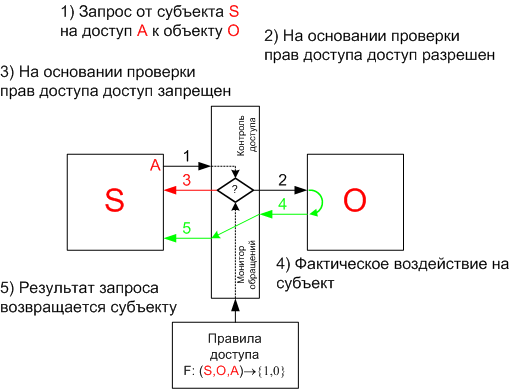
\includegraphics[height=.8\textheight]{pict/AccessControl} }
        \mode<article>{ 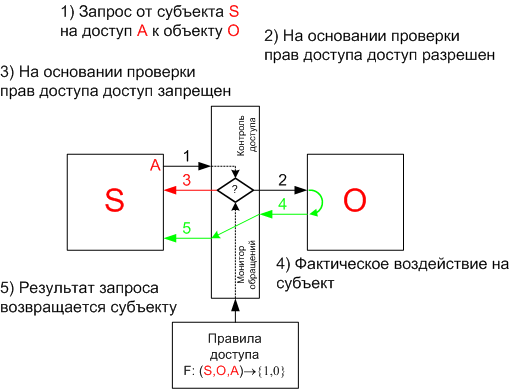
\includegraphics[width=.8\textwidth]{pict/AccessControl} }
    \end{center}
\end{figure} 
\end{frame}


Подразумевается активная система контроля, через которую проходят все запросы на доступ субъектов к объектам. Реализуется часто как компонент операционной системы --- монитор обращений. Попытки субъекта получить доступ в обход системы защиты должны ей подавляться (пример – прикладная программа не может выполнять низкоуровневые операции ввода-вывода). Отсюда вывод – система контроля доступа работает (может быть реализована) в архитектуре клиент-сервер на стороне сервера. 
Монитор обращений имеет следующую структуру:

Различают несколько моделей систем контроля доступа:
\begin{itemize}


\item Discretionary access control (DAC). 

Дискреционные или избирательные. Субъект-владелец объекта полностью контролирует доступ к нему со стороны других субъектов. Для реализации модели этой системы контроля необходимо соблюдение следующих требований: 

\begin{itemize}
\item все субъекты и объекты системы должны быть идентифицированы; 
\item права доступа субъекта к объекту системы определяются на основании некоторого внешнего по отношению к системе правила (свойство избирательности). 
\end{itemize}

Используется принцип: что не разрешено --- то запрещено. Наиболее простой пример дискреционной модели – матрица доступа. По строкам матрицы располагаются субъекты, а по столбцам --- объекты. В ячейках матрицы находятся записи о правах доступа (чтение, запись, удаление и пр.)
Избирательная политика безопасности наиболее широко применяется в коммерческом секторе, так как ее реализация на практике отвечает требованиям коммерческих организаций по разграничению доступа и подотчетности, а также имеет приемлемую стоимость и небольшие накладные расходы. Недостатки данной системы в том, что есть вероятность получения доступа к конфиденциальной информации, так как такое её состояние в терминах модели не определено вообще. Пользователь должен обладать дополнительными знаниями о системе безопасности. Организовать аудит в такой системе сложнее, чем в остальных.


\item Mandatory access control (MAC). 

Мандатные или полномочные. При проверке полномочий важен мандат субъекта, а не сам субъект. Для всех субъектов, имеющих правомочный мандат, доступ будет открыт.
Для реализации этой модели необходимо соблюдение следующих требований:
\begin{itemize}
\item все субъекты и объекты системы должны быть однозначно идентифицированы;
\item задан линейно упорядоченный набор меток секретности;
\item каждому объекту системы присвоена метка секретности, определяющая ценность содержащейся в нем информации;
\item каждому субъекту системы присвоен уровень прозрачности, определяющий максимальное значение метки секретности объектов, к которым субъект имеет доступ
\end{itemize}

Основное назначение такой системы контроля --- регулирование доступа субъектов системы к объектам с различным уровнем критичности и предотвращение утечки информации с верхних уровней должностной иерархии в нижние, а также блокирование возможного проникновения с нижних уровней в верхние.
Достоинство --- более высокая степень надежности, правила ясны и понятны.
Недостатки --- реализация систем с политикой безопасности данного типа довольно сложна и требует значительных ресурсов вычислительной системы. Распространена в системах военного назначения, где имеется четкое разделение информации по грифам секретности. Поэтому в коммерческом секторе применения находит редко.

\item Role-based access control (RBAC). Ролевые. 

Основывается на разграничении доступа к объектам системы на основе их организационной принадлежности, функциям, т.е. ролям выполняемым в системе.

\end{itemize}


К какому виду систем контроля относится система контроля доступа к памяти, выполнения привилегированных команд, доступа к портам ввода-вывода?


\subsection{Аудит}

Протоколирование попыток доступа позволяет отслеживать действия пользователей,  реконструировать прошедшие события и выявлять в реальном масштабе времени угрозы безопасности до их реализации.

\begin{frame}
\frametitle{Аудит}
\begin{definition}%theorem, lemma, proof, corollary, example
\alert{Аудит} --- это протоколирование воздействий субъекта на объект
\end{definition}
В рамках аудита происходит сбор как минимум следующей информации о воздействии.
\begin{itemize}
    \item Идентификатор субъекта (пользователя, процесса) --- инициатора события.
    \item Имена (идентификаторы) затронутых объектов.
    \item Тип, дата, время и результат события.
    \item Источник запроса события.
    \item Описание изменений касающихся механизмов защиты (Вход в систему и выход из нее; Смена атрибутов безопасности).
    \item Метки безопасности субъектов и объектов события.
\end{itemize}
\end{frame}

Перечень событий и фиксируемых атрибутов события определяется принятой политикой безопасности. Активный аудит --- это отслеживание подозрительных действии в реальном масштабе времени. Активный аудит используют системы обнаружения вторжений (Intrusion detection systems) и системы противодействия вторжениям (Intrusion prevention systems). Обычно активный аудит включает выявление нетипичной активности субъектов и выявление начала злоумышленных действий по имеющейся статистике и сигнатурам известных атак.


\section{Стандарты информационной безопасности}


\subsection{Зарубежные и международные стандарты}

\begin{frame}
\frametitle{Зарубежные и международные источники стандартов}
Во развитых странах были сформулированы собственные срандарны информационной безопасности. <<Законодателями мод>> являются следующие организации, комитеты и агентства:
\begin{itemize}
    \item British Standards Institution (BSI);
    \item National Institute of Standards and Technology (NIST);
    \item North American Electric Reliability Corporation (NERC);
    \item International Organization for Standardization (ISO);
    \item International Electrotechnical Commission (IEC);
    \item World Wide Web Consortium (W3C);
    \item Internet Engineering Task Force (IETF);
    \item International Telecommunication Union (ITU);
\end{itemize}
В России стандартизацией занимается Федеральное агентство по техническому регулированию и метрологии.
\end{frame}


Фундаментальным стандартом является британский стандарт BS 7799. Его первая часть легла в основу наиболее популярного ныне стандарта ISO/IEC 17799, а затем и в стандарт ISO/IEC 27002.


\begin{frame}
\frametitle{Международные стандарты ISO/IEC}
Наибольшее распространение получили стандарты тандема ISO/IEC. Основные направления, охваченные стандартами ISO/IEC.
\begin{itemize}
    \item Evaluation criteria for IT security (\alert{ISO/IEC 15408-1, ISO/IEC 15408-2, ISO/IEC 15408-3}).
    \item Code of practice for information security management (\alert{ISO/IEC 27002, заменил ISO 17799}).
    \item Information security management systems (\alert{ISO/IEC 27000, ISO/IEC 27001, ISO/IEC 27003, ISO/IEC 27004}).
    \item Management of information and communications technology security (MICTS) (\alert{ISO/IEC 13335-1, ISO/IEC 27005}).
    \item Guidelines for the management of IT security (GMITS) (\alert{ISO/IEC 13335-2, ISO/IEC 13335-3, ISO/IEC 13335-4, ISO/IEC 13335-5})
\end{itemize}
\end{frame}


Кроме того, стандарты ISO/IEC оговаривают вопросы создания фреймворков для обеспечения безопасности, безопасности сетей, процессов аутентификации, алогритмов шифорвания, алгоритмов получения хеш-функций и цифровых подписей, протоколов управления ключами.


\begin{itemize}
    \item Evaluation criteria for IT security. Критерии оценки безопасности IT. Так называемые <<общие критерии>>. Состоит из трех частей: Введение и общая модель (ISO/IEC 15408-1 Introduction and general model), Функциональные требования (ISO/IEC 15408-2 Security functional requirements), Требования доверия к безопасности (ISO/IEC 15408-3 Security assurance requirements).
    \item Code of practice for information security management. Практические правила управления информационной безопасностью (ISO/IEC 27002, заменил ISO 17799).
    \item Information security management systems. Системы управления информационной безопасностью. Основы и определения (ISO/IEC 27000 Fundamentals and vocabulary), Требования (ISO/IEC 27001 Requirements), Руководство по реализации (ISO/IEC 27003 implementation guidance), Измерения (ISO/IEC 27004 measurements).
    \item Management of information and communications technology security (MICTS). Концепция и модели управления безопасностью информационных и телекоммуникационных технологий. Концепции (ISO/IEC 13335-1), Упрвление рисками (ISO/IEC 27005).
    \item Guidelines for the management of IT security (GMITS). Методы управления безопасностью информационных технологий. Управление и планирование безопасностью (ISO/IEC 13335-2), Технологии для управления безопасностью (ISO/IEC 13335-3), Выбор гарантий (ISO/IEC 13335-4), Управление сетевой безопасностью (ISO/IEC 13335-5)
\end{itemize}


\subsection{Российские ГОСТ'ы}


Российские стандарты основаны большей частью на международных стандартах. Это распространенная практика во многих странах мира. Впрочем, есть и специфичные стандарты.


\begin{frame}
\frametitle{Стандарты Российской Федерации}
Российским аналогом стандарта ISO/IEC 15408 является ГОСТ Р ИСО/МЭК 15408 от 2008 года.

\alert{Информационная технология. Методы и средства обеспечения безопасности. Критерии оценки безопасности информационных технологий.}
\begin{itemize}
    \item ГОСТ Р ИСО/МЭК 15408-1-2008. Часть 1. Введение и общая модель;
    \item ГОСТ Р ИСО/МЭК 15408-2-2008. Часть 2. Функциональные требования безопасности;
    \item ГОСТ Р ИСО/МЭК 15408-3-2008. Часть 3. Требования доверия к безопасности.
\end{itemize}
\end{frame}


\begin{frame}
\frametitle{Стандарты Российской Федерации}
Части Российского ГОСТ Р ИСО/МЭК 13335 также являеются переводом соответствующих стандартов ISO/IEC.

\alert{Информационная технология. Методы и средства обеспечения безопасности.}
\begin{itemize}
    \item ГОСТ Р ИСО/МЭК TO 13335-1-2006. Часть 1. Концепция и модели менеджмента безопасности информационных и телекоммуникационных технологий;
    \item ГОСТ Р ИСО/МЭК ТО 13335-3-2007. Часть 3. Методы менеджмента безопасности информационных технологий;
    \item ГОСТ Р ИСО/МЭК ТО 13335-4-2007. Часть 4. Выбор защитных мер;
    \item ГОСТ Р ИСО/МЭК ТО 13335-5-2006. Часть 5. Руководство по менеджменту безопасности сети.
\end{itemize}
\end{frame}


\begin{frame}
\frametitle{Стандарты Российской Федерации}
Несколько устаревшему ISO 17799 (заменен стандартом ISO/IEC 27002) соответствует \alert{ГОСТ Р ИСО/МЭК 17799-2005}. Кроме того, имеются специфичные ГОСТ:
\begin{itemize}
    \item ГОСТ Р 50922-2006. Защита информации. Основные термины и определения;
    \item ГОСТ Р 53114-2008. Защита информации. Обеспечение информационной безопасности в организации. Основные термины и определения;
    \item ГОСТ 28147-89. Системы обработки информации. Защита криптографическая. Алгоритм криптографического преобразования;
    \item ГОСТ Р 34.10-2001. Информационная технология. Криптографическая защита информации. Процессы формирования и проверки электронной цифровой подписи.
\end{itemize}
\end{frame}


\section{Лицензирование деятельности в области ИБ}


\begin{frame}
\frametitle{Лицензирование}
Согласно постановлению от 26 января 2006 г. N 45 <<Об организации лицензирования отдельных видов деятельности>>, принятого в соответствии с федеральным законом <<О лицензировании отдельных видов деятельности>> следующие федеральные органы исполнительной власти осуществляют лицензирование в области информационной безопасности:

\begin{itemize}
    \item \alert{ФСТЭК} --- Федеральная служба по техническому и экспортному контролю;
    \item \alert{ФСБ} --- Федеральная служба безопасности.
\end{itemize}
\end{frame}


\begin{frame}
\frametitle{ФСТЭК}
ФСТЭК занимается лицензированием деятельности по технической защите конфиденциальной информации, а также (совместно с ФСБ)деятельности по разработке и (или) производству средств защиты конфиденциальной информации (СЗКИ).

На сайте ФСТЭК (см. \cite{bib:fstec}) можно найти соответствующие реестры и перечни:
\begin{itemize}
    \item лицензий на деятельность по технической защите конфиденциальной информации и на деятельность по разработке и (или) производству СЗКИ;
    \item сертифицированных средств защиты информации;
    \item органов по сертификации;
    \item испытательных лабораторий.
\end{itemize}
\end{frame}


\begin{frame}[allowframebreaks]
\frametitle{ФСБ}
ФСБ (см. \cite{bib:fsb}) занимается лицензированием следующих видов деятельности.
\begin{itemize}
    \item Разработка, производство, реализация и приобретение в целях продажи специальных технических средств, предназначенных для негласного получения информации, индивидуальными предпринимателями и юридическими лицами, осуществляющими предпринимательскую деятельность.
    \item Деятельность по выявлению электронных устройств, предназначенных для негласного получения информации, в помещениях и технических средствах (не для собственных нужд).
    \item Деятельность по распространению криптографических средств.
    \item Деятельность по техническому обслуживанию криптографических средств.
    \item Предоставление услуг в области шифрования информации.
    \item Разработка, производство криптографических средств, защищенных с использованием криптографических средств информационных систем, телекоммуникационных систем.
\end{itemize}
\end{frame}


\begin{frame}
\frametitle{Центр <<ЛСЗ>> ФСБ России}
Центр по лицензированию, сертификации и защите государственной тайны ФСБ России (Центр <<ЛСЗ>> ФСБ России, см. \cite{bib:clsz}) в структуре органов федеральной службы безопасности является головным подразделением, уполномоченным на организацию и осуществление лицензирования деятельности предприятий, учреждений и организаций.

Центр <<ЛСЗ>> ФСБ России также организует сертификацию СЗИ и аккредитацию испытательных лабораторий (соответствующие реестры и перечни можно найти в \cite{bib:fsb}). 
\end{frame}

\appendix

\begin{frame}[allowframebreaks]{Библиография}
    \bibliographystyle{gost780u}
    \bibliography{./../bibliobase}
\end{frame}


\end{document}